
\subsection*{First Calculations}
\subsubsection*{Assumptions}
Assumptions used:

\begin{enumerate}[label=\roman*.]
\item$\mu = 0$ (no slip boundary condition)
\item$\rho =constant$ (fluid is incompressible)
\item Control volume: $1\rightarrow 2\rightarrow3\rightarrow 4$ (uniform flow)
\item Immediately above and immediately below rotor blade: points 2,3 respectively
\item Induced velocity from rotor: $v_2=v_3=v_i$ (no velocity jump across disc)
\item Rotor blade assumed to be thin disc when in rotation
\item Pressure jump between sections 2 and 3 $(p2 \neq p3)$
\item $p_1=p_4=p_\infty$
\item Quasi-Steady flow
\item 1-D flow
\item Rotor treated as thin actuator disc
\item Quiescent flow outside of C.V.
\item $ Tip losses=0$   \\ 
 $\displaystyle{T.L.F=B=1-\frac{1.386\lambda_i}{N_b}}$   \\
 where $\displaystyle{\lambda_i=\frac{v_i}{v_tip}=\frac{v_i}{\Omega R}}$ , $N_b$= number of rotor blades
\item $A1>>A4$ and $v1<<v4$
\end{enumerate}

\begin{figure}[h!]
\begin{center}
  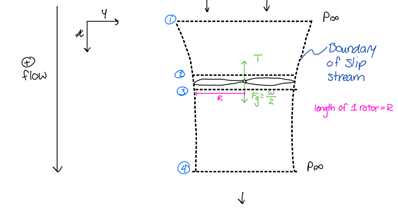
\includegraphics[scale=1]{Pictures/part1_fig1.png}
  \caption{Control surfaces in controlled volume and x-y coordinate system set for 1 rotor where $T = thrust$ and $F_g= gravitational force of blade$ (replace sketch?)}
    \label{fig:part1_fig1}
\end{center}
\end{figure}
\FloatBarrier
*Let CS = CSI + CSIII + ....... (Lumped CS)

\subsubsection*{Conservation of mass}
Using the conservation of mass, the mass flow rate through the boundary surfaces 1 and 4 is:
\begin{equation}
\frac{dM}{dt}\bigg|_s= \dot{m}_4 - \dot{m}_1 = 
\frac{\delta}{\delta x} \iiint\limits_{CV}\rho dV +\iint\limits_{CS} \rho  \overrightarrow{v}d \overrightarrow{A} 
\end{equation}

From assumption (ix): Quasi-steady, so $\iiint\limits_{CV}\rho dV = 0$
Expression (1) now becomes 
$$ \frac{dM}{dt}\bigg|_s= \dot{m}_4 - \dot{m}_1 =0 $$

Since the mass flow rates across all boundaries are equivalent:
\begin{align}
\dot{m}_1 = \dot{m}_2 &= \dot{m}_3 = \dot{m}_4 \\
\dot{m}_i &= \rho A_i\ v_i
\end{align}

\subsubsection*{Conservation of momentum}
The momentum equation for the inertial volume is:
\begin{equation}
\sum F\big|_s= 
\frac{\delta}{\delta x} \iiint\limits_{CV}\rho \overrightarrow{v} dV +\iint\limits_{CS} \overrightarrow{v}\rho  \overrightarrow{v}d \overrightarrow{A} 
\end{equation}
Momentum components in x,y directions, see fig X for system sketch: $ \overrightarrow{F}_y =0  $ (no forces in y direction)
\begin{align}
\sum F = T - \frac{W}{2} = 0\\
-R_x = T = \frac{W}{2} =  \dot{m}_4 \dot{v}_4 -  \dot{m}_1 \dot{v}_1
\end{align}
From assumption (xiv)
\begin{equation}
T = \frac{W}{2} =  \dot{m}_4 \dot{v}_4
\end{equation}
\subsubsection*{Conservation of energy}
\begin{equation}
\dot{Q} - \dot{W} =
\frac{dE}{dt}\bigg|_s= \dot{m}_4 - \dot{m}_1 = 
\frac{\delta}{\delta x} \iiint\limits_{CV}e \rho dV +\iint\limits_{CS} e\rho  \overrightarrow{v}d \overrightarrow{A} 
\end{equation}

where $e=u+\frac{P}{\rho}+\frac{v^2}{2}+gz $ and $\dot{W}=\dot{W}_{Shaft}+\dot{W}_{normal \, stress}+\dot{W}_{others}$
From assumption (ix) and since the system is isothermal we get:













